\chapter{Нейрофизиология и астрономия в качестве областей с интенсивным использованием данных} \label{chapt3}

\section{Задачи по анализу сигналов фМРТ в нейрофизиологии}\label{sect_4_1}
\subsection{Введение}
Для сообщества, занимающегося нейронаукой, разработка общих парадигм исследования огромного числа функциональных систем в головном мозге все еще остается труднейшей задачей. Построенный на термине коннектом, изобретенном для описания подробной карты соединений нейронов в мозге человека, термин функциональный коннектом обозначает совокупное множество функциональных соединений в мозге (его схему коммутации) \cite{biswal2010toward}. В более широком смысле коннектом включает в себя отображение всех нейронных соединений нервной системы организма. Вопросы образования и изучения коннектома, известные как коннектомика, могут простираться по своему масштабу от детальной карты полного набора нейронов и синапсов в пределах части или всей нервной системы организма до описания макромасштабных процессов \cite{craddock2013imaging} функциональной и структурной межнейронной коннективности между всеми полями коры головного мозга и субкортикальными структурами. Конечная цель коннектомики "--- картирование мозга человека. В функциональной магниторезонансной томографии (fMRI "--- фМРТ) считается, что визуализируемые соединения представляют собой функциональную связность в том смысле, что две области мозга совместно участвуют в реализации некоторой более высокого порядка функции, нередко в контексте выполнения определенной задачи. 

Технология fMRI стала мощным инструментом, используемым для изучения многочисленных функциональных схем одновременно. Это привлекло к себе внимание статистиков, работающих в этой сфере. На уровне элементарных измерений данные нейровизуализации могут, в основном, рассматриваться как состоящие из ряда сигналов (как правило, последовательных во времени) в каждой совокупности пикселей (в двух измерениях) или вокселей (в трех измерениях). Исходя из этих данных, нейровизуализация использует различные формы представления информации более высокого уровня. За последние годы в нейровизуализации возник существенный интерес к представлениям на основе сетей, где сети (графы) используются для обобщения информации о связях в множестве измерений, обычно предполагающих отражение функциональных или структурных отношений между исследуемыми областями мозга. Нетрудно предсказать, что поскольку нейровизуализация стала теперь стандартным инструментом клинической нейронауки, мы быстро движемся к моменту, когда в нашем распоряжении окажутся доступные базы данных, состоящие из больших массивов вторичной информации в виде объектов данных на основе сетей. 

Одной из наиболее фундаментальных задач, представляющих интерес в анализе таких данных, является проверка гипотез, отвечающих на такие вопросы, как Есть ли разница между сетями (графами) этих двух групп объектов?. Сети не являются эвклидовыми объектами, и поэтому классические методы статистики здесь нельзя применять непосредственно. Аналоги классических инструментов оценки (на основе статистики) и проверки гипотез исследуются в \cite{ginestet2017hypothesis, ginestet2014statistical}. Такое исследование мотивировано проектом 1000 функциональных коннектомов (1000 FCP), запущенном в 2010 г. \cite{biswal2010toward}. Проект 1000 FCP \cite{yan2013standardizing} включает в себя самое большое множество данных такого рода, сходного с большими множествами данных в генетике. В проект 1000 FCP включено описание данных функциональной нейровизуализации 1093-х субъектов, находящихся в 24-х центрах сообщества. Средний возраст участников "--- 29 лет, а все субъекты были возрастом 18 лет или старше.


Другие проекты (такие как проект Коннектом человека (Human Connectome Project "--- HCP) \cite{VanEssen2013}) имеют целью построить сетевую карту (граф) мозга здорового, живого взрослого человека.
 Суммарный объем данных, выдаваемых проектом HCP, будет, по-видимому, составлять много петабайтов \cite{VanEssen2013}. Из информатики платформа HCP включает в себя как платформу систему управления данными ConnectomeDB на базе платформы визуализации XNAT из той же информатики \cite{marcus2007extensible}, широко используемую систему с открытым кодом для управления и совместного пользования данными визуализации и взаимосвязанными данными. В настоящее время проект HCP располагает информацией о более чем 1000 субъектам, включая структурные сканы (\textit{T1w} и \textit{T2w}), fMRI в покое (rfMRI), fMRI действия (tfMRI) при выполнении задачи, а также диффузионная визуализация МРТ (dMRI) с высокой угловой разрешающей способностью. Кроме того, доступны данные MEG в покое (rMEG) и/или данные MEG (tMEG) при выполнении задачи. Данные поступают в нескольких форматах: необработанные сырые данные, предварительно минимально обработанные, а также наборы данных по результатам анализа. В предварительно обработанных наборах данных пространственные нарушения минимальны, а данные были выровнены по их модальностям и по субъектам с использованием соответствующих методов регистрации по объемам и по поверхностям. Сообщество исполнителей проекта HCP рекомендует пользоваться предобработанными наборами данных. 

Можно ожидать, что в ближайшем будущем в нейронауке появится большое количество баз данных сетевых объектов, мотивирующих разработку и расширение различных инструментов от классической статистики до глобальных сетевых данных.

Исследование функциональной связности с помощью fMRI широко используется, так как метод обладает высоким пространственным разрешением, анализ проводится интактно, не требуя инъекций или хирургических вмешательств. Данные fMRI представляют собой 4-х мерные изображения (одна временная координата и три пространственных) и предназначены для регистрации гемодинамических реакций головного мозга, вызванных активностью нейронов. Различают два типа fMRI: 1) изображения fMRI, которые были получены, когда человек находился в состоянии покоя, то есть во время проведения эксперимента испытуемого просили закрыть глаза, расслабиться и ни о чем не думать; 2) изображения fMRI, которые были получены во время некоторого действия, например, у испытуемого стимулируется проявление эмоций, зрительных или двигательных реакций и пр. Изображения fMRI имеют сложную структуру и требуют больших ресурсов для их хранения, таких как высокопроизводительные вычислительные системы. 

% TODO типы взаимодействия
%Существует три типа взаимодействия между регионами головного мозга: структурное, эффективное и функциональное. 
Исследование функциональной связности в состоянии покоя имеет существенное значение, так как полученные результаты позволяют выделять нейросети покоя и анализировать их активность. Другим примером связности является эффективная связность. Анализ эффективной связности показателей fMRI действия позволяют оценить участие конкретных структур мозга в обеспечении сложных функций, таких как язык, память, азартная игра, движения. Эти подходы используются для изучения когнитивных и других функций мозга, а также для исследования различных заболеваний: болезни Паркинсона, синдром дефицита внимания/гиперактивности, болезни Альцгеймера и др. Задачи исследования различных типов связности являются актуальными и представляют существенный интерес.

\subsection{Выделение регионов головного мозга из fMRI изображений}

Визуализация, обработка и анализ многомерных данных, таких как изображения, часто требует некоторой предварительной обработки, для того чтобы уменьшить размерность данных и получить отображение исходно представленных данных на низкоразмерное векторное пространство. Предположение таково, что исходные данные находятся в низкоразмерном подпространстве или многообразии \cite{brun2006manifold}, вложенном в исходное пространство. Эта часть исследований называется сокращением размерности, или нелинейным сокращением размерности, включающей в себя методы параметризации данных с использованием низкоразмерных многообразий (манифольдов) в качестве моделей. В сообществе обработчиков информации по нейронам это известно под названием обучения на базе многообразий. Методы обучения на базе многообразий дают возможность отыскивать нелинейные параметризации многообразий информационных точек, находящихся в высокоразмерных пространствах, весьма сходно с тем, как метод главных компонент (МГК) способен узнавать или выявлять наиболее важное линейное подпространство набора информационных точек (проецируя данные на $n$-размерное линейное подпространство, которое дает максимум дисперсии распределения вероятностей данных в новом пространстве). Такие преобразования называются выделением регионов головного мозга человека.

В качестве переменных для построения зависимостей используются регионы головного мозга (ROI). ROI — это набор анатомически близких вокселей, которые представляют собой встроенные единицы изображения МРТ, представляющие маленькие кубики мозга. Поскольку изображение МРТ фиксирует изменения во времени уровня кислорода в крови, каждый воксель связан с соответствующим временным рядом. ROI также связаны с временными рядами, например, усредненными по всем временным рядам его вокселей. На данном этапе требуется преобразовать 4-х мерное изображение головного мозга в двухмерный массив (регионы головного мозга – время). Выделение регионов можно рассматривать как один из способов уменьшения размерности. При использовании данного подхода регионы некоторым образом группируются и усредняются, а само усредненное значение является представительным значением для данного региона. Также при использовании данного метода делается предположение, что воксели одного региона ведут себя схожим образом. 

Существует множество методов для выделения регионов головного мозга \cite{Arslan2018}. Все методы можно разделить на три группы:
\begin{enumerate}
    \item Выделение регионов для одного человека (субъекта);
    \item Выделение для группы людей;
    \item Использование различных атласов головного мозга человека.
\end{enumerate}

Методы первого типа подразделяют поверхность головного мозга каждого субъекта независимо друг от друга. Часть методов в данном подходе основа-на на широко используемых алгоритмах кластеризации, таких как $k$-средних \cite{arslan2015multi}, агломеративной иерархической кластеризации \cite{blumensath2013spatially} и спектральной кластеризации \cite{van2008normalized}. Если набор данных состоит из нескольких субъектов, то первоначально все данные объединяются в один большой набор, состоящий из $M$ субъектов, а затем применяются МГК/МНК.

При больших наборах данных или при большом количестве субъектов становится неразумным формировать полный набор данных, а затем применять МГК и МНК из-за ограничений по памяти и по вычислительному времени. Для решения этой проблемы было предложено использовать групповые методы. Групповые методы строят репрезентативные модели популяции. Методы получения регионов группового уровня обычно основываются на предположении, что пространственное соответствие между субъектами было обеспечено априори. Следовательно, каждая вершина (или воксель) представляет собой одно и то же пространственное положение для каждого субъекта. Это позволяет объединить или усреднить данные по различным субъектам для анализа на популяционном уровне. Существует два наиболее популярных способа.

Первым способом является вычисление регионов для каждого субъекта индивидуально, а затем применение второго уровня алгоритма кластеризации на уровне популяции (т. е. двухуровневый подход). Двухуровневый подход обеспечивает группировку вокселей одних и тех же регионов вместе. В результате регионы группового уровня, полученные с помощью этого метода, выражают общие характеристики популяции, аппроксимируемые регионами, полученные для каждого субъекта в отдельности. Примером является применение двухуровненого применение метода главных компонент \cite{calhoun2001method} (см. \cref{fig:two_step_pca}). Сначала каждый набор данных сокращается до $\rho$ основных пространственных векторов с использованием МГК, а затем объединив их и применив еще раз  МГК, чтобы уменьшить конечный набор данных до $k$ компонент.

\begin{figure}[ht]
    \centering
    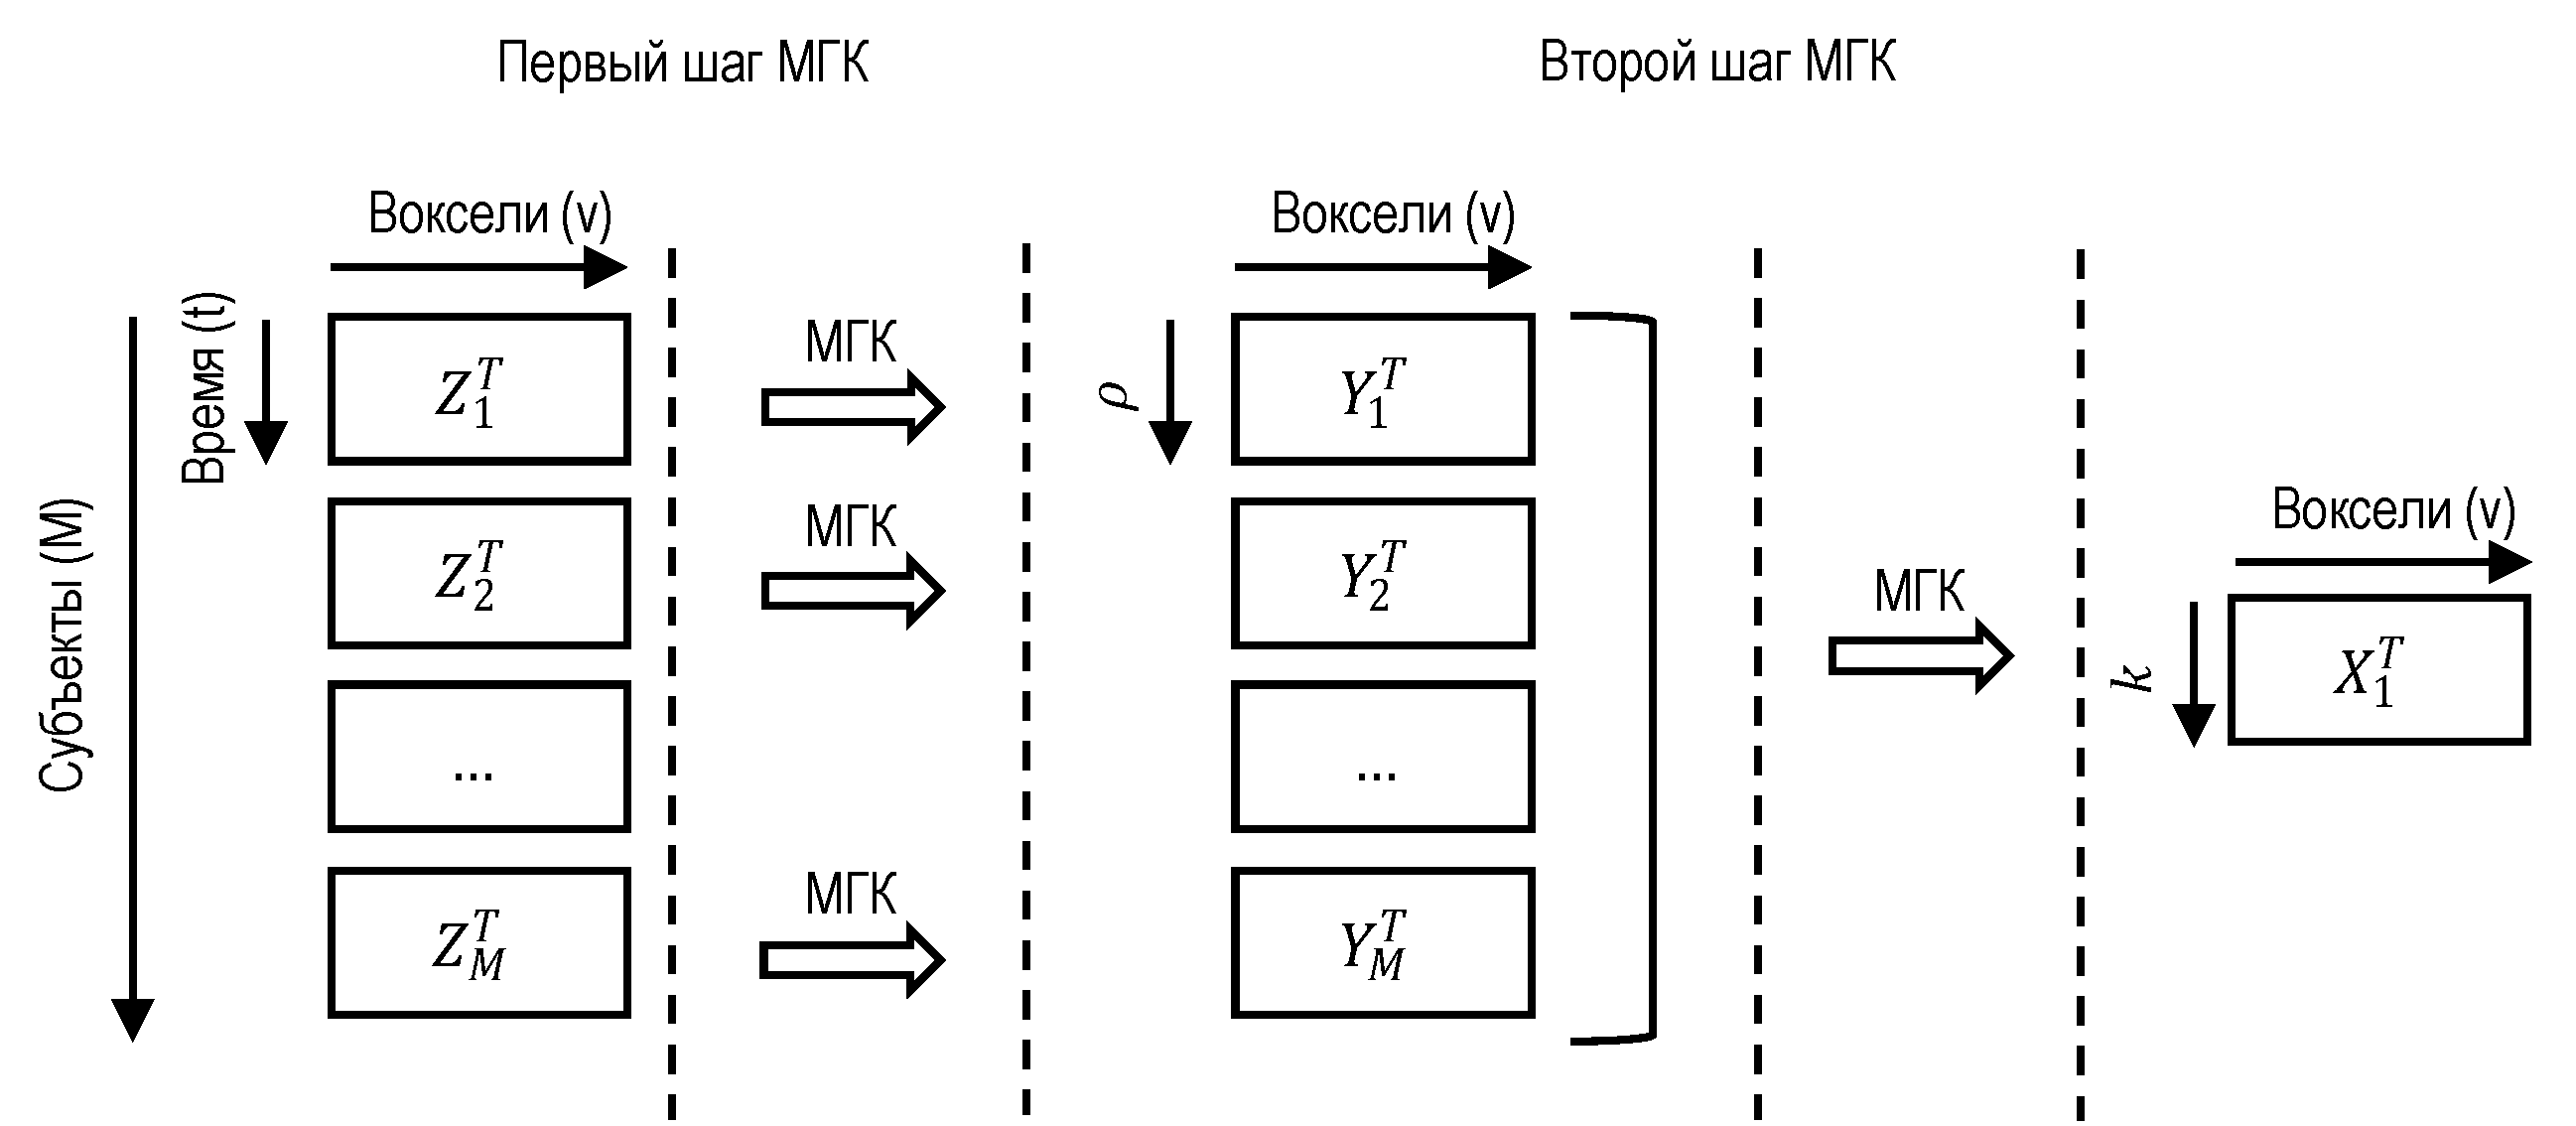
\includegraphics[width=1.0\linewidth]{images/two_step_pca.pdf}
    \caption{Двухуровненое применение метода главных компонент.}\label{fig:two_step_pca}
\end{figure}

Хотя использование небольшого значения $m$ ограничивает требования к памяти для этих операций, размер данных масштабируется линейно с количеством объектов, которые в конечном итоге могут стать непрактично большими. Кроме того, важная часть информации может быть потеряна, если $m$ не является относительно большим (обычно оно не должно быть большим). Информацию может быть трудно оценить на уровне отдельного субъекта, но она может быть важна на уровне группы. 

Вторым способом является вычисление репрезентативной матрицы признаков из популяции, например, путем объединения временных рядов и далее подходу группового среднего. Данный метод направлен на поиск общих паттернов между индивидами в пределах популяции путем вычисления группового среднего представления, что достигается путем объединения временных рядов каждого субъекта и применения метода главных компонент или его модификаций для уменьшения размерности для выделения регионов (см. \cref{fig:group_pca}). Широко используемым является алгоритм MELODIC Incremental Group-PCA (MIGP) \cite{rachakonda2016memory} . MIGP "--- это инкрементный подход, целью которого является обеспечение очень близкого приближения к полной конкатенации набора данных, за которым следует МГК, но без больших требований к памяти. Высокая точность достигается за счет того, что отдельные наборы данных субъектов не сводятся к небольшому числу компонентов МГК. Инкрементный подход сохраняет внутреннее пространство МГК из $m$ взвешенных пространственных собственных векторов, где $m$ обычно больше, чем количество временных точек в каждом отдельном наборе данных. Под "взвешенным" подразумевается, что собственные значения включены в матрицу пространственных собственных векторов. Конечный набор из $m$ компонентов, представляющих временно объединенные выходные данные МГК, затем может быть уменьшен до требуемого размера $n$ просто путем сохранения верхних $n$ компонентов и, при необходимости, отбрасывания весовых коэффициентов (собственных значений).

Обычно сначала объединяются 2-3 субъекта. Затем этот набор данных вводится в $m$-мерный объект и получается следующая матрица. Каждый вектор умножается на свое собственное значение. Собственные значения характеризуют важность компонента здесь, поэтому статистическая информация не теряется и сохраняется дисперсия каждого субъекта. MIGP не увеличивает требования к памяти с увеличением числа объектов, большие матрицы никогда не формируются, а время вычисления линейно зависит от количества объектов.

\begin{figure}[ht]
    \centering
    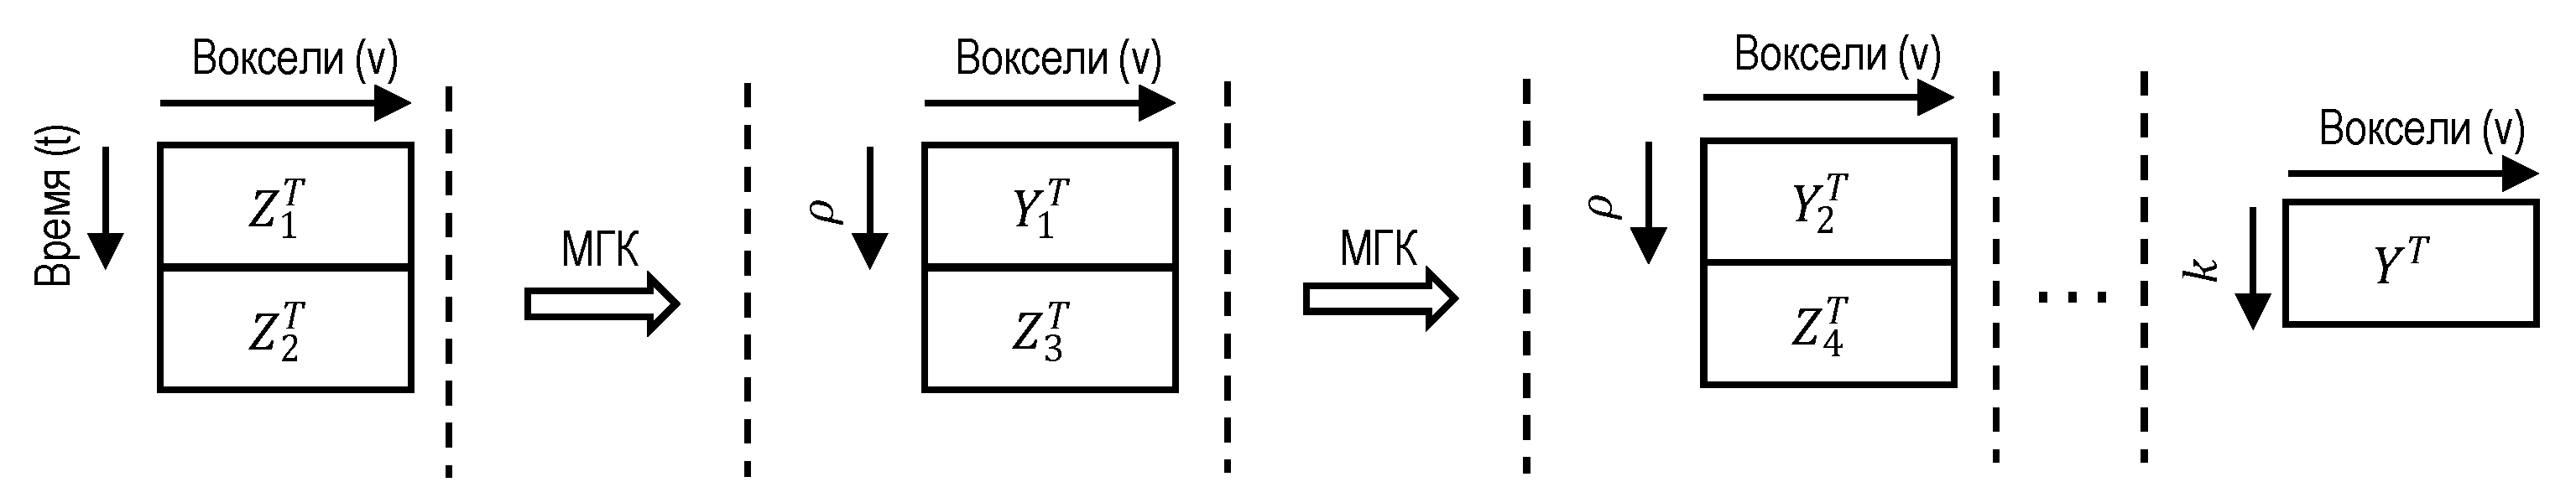
\includegraphics[width=1.0\linewidth]{images/group_pca.pdf}
    \caption{Последовательное применение метода главных компонент.}\label{fig:group_pca}
\end{figure}

При работе с атласами головного мозга человека используется заранее вычисленная функция, ставящая каждому вокселю изображения в соответствие регион головного мозга. Существует множество атласов головного мозга человека, например, вероятностный атлас Harvard-oxford \cite{desikan2006automated}, в котором описано 48 кортикальных регионов и 23 субкортикальных. В работе \cite{fischl2004automatically} проводились ряд экспериментов по результатам которых делается вывод об оптимальном количестве структурных регионов. Проведен сравнительный анализ на нескольких наборах данных между ручной разметкой и при помощи атласа Destrieux 2009. Авторы статьи утверждают, что оптимальное количество регионов в атласе 150–160, при таком количестве удаться достичь баланс между размерностью данных и качеством извлекаемого сигнала. Automated Anatomical Labeling (AAL) атлас является результатом автоматической анатомической маркировки пространственно нормализованного набора данных фМРТ высокого разрешения, предоставленного Монреальским неврологическим институтом (MNI). Данный атлас включает 116 структурных областей головного мозга \cite{tzourio2002automated}.

 
\subsection{Анализ функциональной связности линейными и нелинейными методами}
Существует два типа функциональной связности головного мозга человека: линейная и нелинейная. В большинстве случаев исследуется лишь линейная функциональная связность. Хотя линейная модель проста и полезна в некоторых исследованиях \cite{soch2017improve, eklund2017bayesian, kovalev2017search}, однако использование лишь линейных функций является сильным ограничением. Так, в работах \cite{lahaye2003functional, karanikolas2016multi} показано, что функциональная связность между некоторыми областями мозга является нелинейной, что показывает актуальность проблемы исследования нелинейной функциональной связности. Одним из способов изучения нелинейной функциональной связности является построение и исследование аналитических функций, как, например, в статье \cite{allgaier2015nonlinear}, где авторы строят аналитические функции с помощью генетического программирования (ГП) и на основе полученных результатов делают выводы о взаимосвязях тех или иных регионов.


Обобщенная линейная модель является одним из популярных методов изучения нейрофизиологических изображений \cite{lahaye2003functional, karanikolas2016multi}. Из всех рассматриваемых методов обобщенная линейная модель является наименее трудно вычислимой, а полученный результат достаточно просто интерпретируется. При этом для поиска нелинейной функциональной связности метод требует модификации. Между двумя регионами головного мозга экспертом определяется некоторая нелинейная функция, которая отображает нелинейное взаимодействие между значениями регионов и подается в качестве входного значения для линейной модели. Недостатком метода является то, что нужно определять такие нелинейные зависимости заранее.

Для автоматического восстановления нелинейных функциональных связей также используется метод генетического программирования. Генетическое программирование не является настолько популярным методом, как обобщенная линейная модель, так как этот метод требователен к вычислительным ресурсам. В работе \cite{allgaier2015nonlinear} авторы показывают применение данного алгоритма, его преимущества и недостатки. Преимуществом является то, что заранее не делается никаких выводов о функциональной связности, как это происходит с обобщенной линейной моделью. Существенным недостатком данного алгоритма является то, что его вычислительная сложность растет экспоненциально с увеличением размерности входных данных. В \cite{Icke2014} предложен модифицированный метод генетического программирования, частично решающий проблему вычислительной сложности. На вход алгоритма подаются функции попарного произведения показателей регионов головного мозга, для которых строится обобщенная линейная модель, для которой отбираются только значимые пары. Отобранные пары затем используются в качестве входных значений для генетического алгоритма. Данный подход демонстрирует лучшие результаты по сравнению с простым алгоритмом генетического программирования. Недостатком такого подхода является то, что, что взаимосвязь между некоторыми регионами может быть потеряна. Также он, в отличие от нейронных сетей, позволяет в явном виде оценить эту связь, так как если даже получится выписать результат для многослойного перцептрона, то он будет сложен для понимания.


\subsection{Поиск значимых различий  функциональной связности головного мозга для разных групп людей в состоянии покоя}


Задача поиска различий в работе головного мозга между мужчиной и женщиной уже давно интересует нейрофизиологов. В начале 2000-х годов появились работы, где показаны сравнение функционирования головного мозга у мужчин и женщин. В статье \cite{koch2007gender} показано, у мужчин и женщин было обнаружено значительное ухудшение показателей рабочей памяти в результате возбуждении отрицательных эмоций. Однако фМРТ-анализ выявил отчетливые различия в активации нейронов. У мужчин когнитивные показатели при возбуждении отрицательных эмоций были связаны с расширенными паттернами активации преимущественно в префронтальной и верхней теменной областях. У женщин взаимодействие между эмоциями и рабочей памятью приводило к значительно более сильной реакции в миндалевидном теле и орбитофронтальной коре. В статье \cite{xu2015gender} показано, что у мужчин и женщин в состоянии покоя есть различия показателей фМРТ в первичной зрительной коре, задней срединной префронтальной сети и других отделов головного мозга. Более того, у мужчин и женщин отличается работа головного мозга во время болезней. В работе \cite{zang2004regional} изучаются различия фМРТ у мужчин и женщин с рассеянным склерозом. Демонстрируется, что при рассеянном склерозе у мужчин проявляется более слабая активность в хвостатом ядре по сравнению с женщинами.

Интересно сравнить субъектно-специфичные сети мужчин и женщин в наборе данных 1000 FCP. В работе \cite{ginestet2017hypothesis} база данных проекта 1000 FCP проводится сравнение сетей, принимая во внимание пол субъектов, по разным возрастным группам, а также по разным местам сбора данных. Показано, что необходим расчет средних значений по каждой подгруппе сетей. Задача была выполнена путем конструирования эвклидовой средней лапласианов для каждой группы субъектов в разных возрастных группах. Такие группо-специфичные средние лапласианы могут в дальнейшем интерпретироваться в каждой группе как средние функциональные коннективности. Такой подход обеспечивает построение тестов для гипотез относительно средних по сетям или группам сетей в целях исследования влияния пола по всем сетям. Что касается набора данных 1000 FCP, тестирование с помощью двухвыборочного критерия для лапласианов производилась относительно того, существенно ли гендерные различия влияют на характерные особенности коннективности мозга. Нулевая гипотеза об отсутствии различий между группами была отброшена. Подобным же образом с высокой вероятность была отвергнута нулевая гипотеза по трем возрастным когортам.

В работе \cite{ginestet2017hypothesis} устанавливаются необходимые математические характеристики, связанные с определенным понятием пространства сетей, используемых для интерпретации функциональной нейровизуализации ориентированных на коннектом данных. Однако расширение инструментов классической статистики на наборы данных на сетевой основе оказалось в высокой степени нетривиальным. Основной трудностью такого расширения оказалось то, что сети не являются эвклидовыми объектами (для которых классические методы и были разработаны) – это, скорее, комбинаторные объекты, определенные ими наборами вершин и ребер. В работе \cite{ginestet2017hypothesis} показано, что сети могут быть связаны с определенными натуральными подмножествами эвклидова пространства, и демонстрируется, что используя сочетание инструментов геометрии, вероятности на многообразиях, а также высокоразмерного статистического анализа, можно разработать основанную на принципах и практическую структуру по аналогии с классическими инструментами. Так, в частности, была разработана асимптотическая структура для тестирования гипотезы, основанной на одной или двух выборках. Ключом к такому подходу является соответствие между неориентированным графом и его лапласианом, где последний определен как матрица (связанная с сетью). Лапласиан графа оказался наиболее подходящим для использования в таких матрицах. Пространство лапласианов графа используется при работе с определенными подмножествами эвклидова пространства, которые являются подмногообразиями стандартного эвклидова пространства.


Недостатком рассмотренных выше работ является применение лишь линейных методов для сравнения регионов (в основном это обычная корреляция Пирсона). При использовании нелинейной функциональной связности становится возможным более подробно исследовать взаимосвязь между регионами головного мозга и лучше понять его работу в целом. В будущем это позволит облегчить поставку диагнозов у мужчин и женщин, а также у людей разного возраста, и диагностировать заболевания на более ранних стадиях и разработать более эффективное лечение. Исследование подходов к поиску значимых различий нелинейной функциональной связности головного мозга для мужчин и женщин в состоянии покоя является актуальной задачей, так как позволит выявить различия с помощью нелинейных методов. При использовании нелинейной функциональной связности становится возможным более подробно исследовать взаимосвязь между регионами головного мозга и лучше понять его работу в целом.
\subsection{Сквозной пример}

В качестве входного набора данных используется 1133 изображения фМРТ покоя проекта HCP. Для каждого человека было проведено по четыре эксперимента. Каждый эксперимент длился 14,4 минуты, временной шаг составлял 0,72 секунды. фМРТ-изображение — это 4D-изображение (пространственные и временные координаты), которое использует формат NIFTI. Каждый воксель имеет физический размер $3\times 3 \times 3$ мм.

В качестве основного алгоритма для построения нелинейной функциональной связности был выбран алгоритм генетического программирования, так как в отличие от алгоритмов с использованием нейронных сетей он является хорошо интерпретируемым, а также не требует построения дополнительных признаков по сравнению с обобщенной линейной моделью.


Для сравнения полученных функций для мужчин и женщин, а также отдельно по возратам, авторами предлагается воспользоваться следующей статистической процедурой:

\begin{enumerate}
    \item Так как известны границы сигнала, то по этим границам выбрать $n$-мерного куба случайные значения, где $n$ "--- это количество регионов минус один.
    \item Для каждого региона сделать следующее:
    \begin{enumerate}
        \item Используя значения, полученные на первом шаге, построить предсказание с использованием функций, построенных отдельно для выбранных групп;
        \item Проверить гипотезу о том, что ошибка для разности между предсказаниями функций отлична от нуля.
    \end{enumerate}
\end{enumerate}

При проверке гипотезы используется ранговый критерий для связных выборок (так как предсказания были получены на одних и тех же значениях). При проверке множественных гипотез используется поправка Холма.


\section{Выводы по главе}\label{sect4_3}

\clearpage